\chapter{Autoencoders}

An autoencoder is a type of Neural Networks designed to learn a compressed or sparse representation of the input data, often referred to as a code or latent space representation. Architecturally wise the network may be viewed as consisting of two parts: an encoder whose goal is to learn a function $f$ that encodes the input data $x$ to a lower-dimensional representation $h=f(x)$ also called hidden or latent space and a decoder that aims to learn a function $g$ able to reconstruct the original input data $x$ from the encoded representation $h$ to the original one $r=g(h)$. Overall, we can see the autoencoder as an architecture aiming to learn the identity function.

$$ x = g(f(x)) $$

\begin{figure}[h]
    \centering
    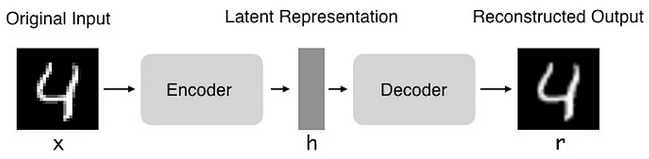
\includegraphics[width=8cm]{Images/autoencoder-architecture.png}
    \caption{Autoencoders architecture}
\end{figure}

\noindent Depending on their configuration autoencoders can be probabilistic or deterministic models.

\begin{itemize}
    \item Deterministic. Both the encoder and the decoder aim is to learn a mapping function $f(x)$ and $g(h)$ respectively. This will mean that for the same input we will always get the same output.
    \item Stochastic. In the stochastic model instead of learning mapping functions our aim is to learn probability distributions given by $p_{encoder} (h | x)$ for the encoder and $p_{decoder} (x | h)$ for the decoder.
\end{itemize}

\begin{figure}[h]
    \centering
    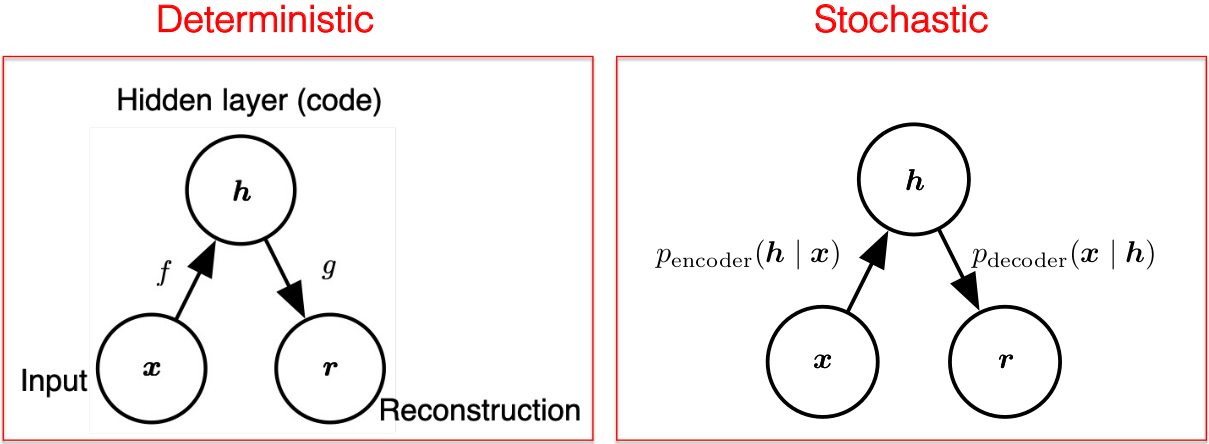
\includegraphics[width=12cm]{Images/autoencoder-det-sto.png}
\end{figure}

\noindent If the only purpose of autoencoders was to learn the identity function on the input domain, they would be useless. Instead, the goal is that the autoencoder learns the underlying structure of the input data. This can be achieved through the imposition of constraints on the replication task making the autoencoder able to learn the underlying structure of the input data.

The specific type of constraints we apply determines whether we are working with an undercomplete autoencoder or an overcomplete autoencoder. An undercomplete autoencoder results from constraints on the network architecture, whereas an overcomplete autoencoder arises from the addition of a regularization term to the loss.



\section{Undercomplete Autoencoders}

In an undercomplete autoencoder, the dimensionality of the encoded representation $h$ is lower than the dimensionality of the input data $x$. By restricting the dimensionality, the undercomplete autoencoder is forced to capture the most important features of the input data in the lower-dimensional representation. This is done by discarding some of the input information when representing the data in the latent space $h$ making the autoencoder unable to exactly reproduce the identity function instead it will try to approximate it. Therefore, the learning process is described simply as minimizing the loss function

$$ L(x, g(f(x)) $$

where $L$ is a loss function penalizing $g(f(x))$ for being dissimilar from $x$, such as the MSE.

\noindent When the autoencoder uses linear units and $L$ is the MSE, an undercomplete autoencoder learns to span the same subspace as PCA (Principal Component Analysis). PCA identifies the principal components, by performing Singular Value Decomposition on the data covariance matrix. The singular vectors corresponding to the largest singular values represent the principal components. These singular vectors form an orthogonal basis that captures the maximum variance in the data.

The goal of a linear autoencoder with MSE loss is to learn a compressed representation of the input data using a linear transformation by minimizing the reconstruction error (which is similar to capturing the variance in the data). The weights learned by the autoencoder in the hidden layer will correspond to the singular vectors of the data covariance matrix, i.e., the principal components. Keep in mind that autoencoders with nonlinear encoder and decoder functions can learn a more powerful nonlinear generalization of PCA, but they also have more risk to overfitting than linear autoencoders.

\begin{figure}[h]
    \centering
    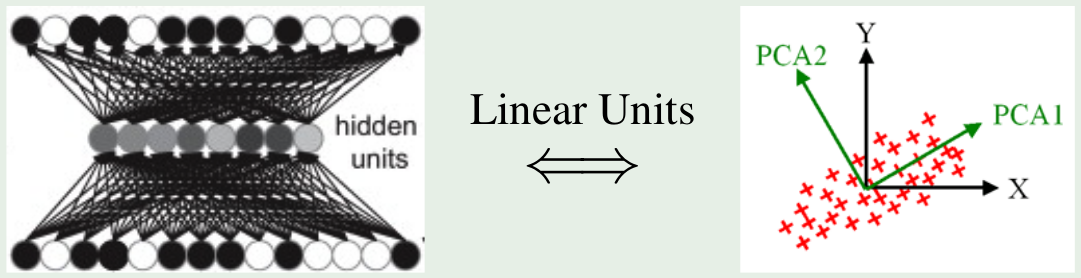
\includegraphics[width=13cm]{Images/pca-autoencoder.png}
    \caption{A shallow autoencoder with linear units is equivalent to performing PCA}
\end{figure}

\subsection{Shallow vs Deep Autoencoders}

From now we have considered the shallow autoencoder case. In this situation, the encoder is used to compress the original data representation into the hidden layer and the decoder uses the data representation in there to return the output. A deep autoencoder has the advantage of learning more complex, non-linear transformations to represent the data. Experimentally, deep autoencoders yield much better compression than corresponding shallow or linear autoencoders. On the other hand they are also more prone to overfitting that shallow autoencoders.

\begin{figure}[h]
    \centering
    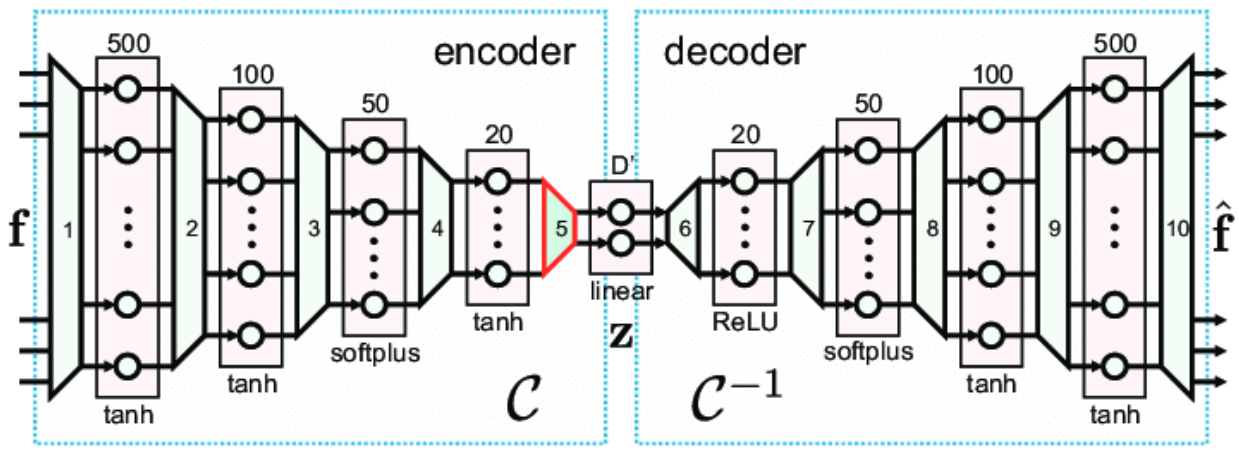
\includegraphics[width=10cm]{Images/deep-autoencoder.png}
    \caption{Deep Autoencoder}
\end{figure}

\section{Overcomplete Autoencoders}

Overcomplete autoencoders work on the opposite direction than undercomplete autoencoders. We no longer have a constrain in the architecture of the network so the latent space representation dimension is usually higher than the original input data dimension. This leads to a more expressive representation at the latent space $h$. But at the same time because overcomplete autoencoders have enough capacity to memorize the entire training set, they will introduce overfitting if not properly regularized. Basically, the autoencoder will just perform the identity function. By adding a regularizing term to the loss function, we will hope to capture the manifold of the underlying representation of the data.

%The function have other properties besides the ability to copy its input to its output. These other properties include sparsity of the representation, smallness of the derivative of the representation, and robustness to noise or to missing inputs. This prevents the autoencoder from simply memorizing the input and instead makes the model learn something useful about the data distribution.

\subsection{Sparse Autoencoders}

A sparse autoencoder is a type of overcomplete autoencoder that incorporates a sparsity constrain by adding a regularization term $\Omega$ to the loss function in addition to the reconstruction error:

$$ L(x, g(f(x))) + \Omega(h) $$

The regularization term $\Omega$ penalizes the hidden representation $h$.  The sparsity constraint encourages the autoencoder to learn a representation where only a small subset of the neurons in the hidden layer is active for any given input. This encourages the autoencoder to learn unique statistical features of the dataset instead of simply acting as an identity function.

\subsection{Denoising Autoencoders}

Rather than adding a penalty $\Omega$ to the cost function, we can obtain an autoencoder that learns the manifold of the underlying structure of the data by changing the reconstruction error term of the cost function. A denoising autoencoder instead minimizes

$$ L(x, g (f ( \hat{x})))$$

\noindent Denoising autoencoders receive as input a corrupted version of the input data and by training the network they are able to reconstruct the original, uncorrupted data input. In order to do that, we will introduce a corruption process $C(\tilde{x} \vert x)$ into our data (noise). The autoencoder then learns a reconstruction distribution $ p_{reconstruct} (\tilde{x} \vert x)  $ estimated from training pairs $ (\tilde{x}, x) $, as follows:

\begin{enumerate}
    \item Sample a training example $x$ from the training data.
    \item Sample a corrupted version $ \tilde{x}$ from $C(\tilde{x} \vert x)$.
    \item Use $ \left( x, \tilde{x} \right) $ as a training example for estimating the autoencoder reconstruction distribution $p_{reconstruct} (x \vert \tilde{x} ) = p_{decoder} (x \vert h)$
\end{enumerate}


\begin{figure}[h]
    \centering
    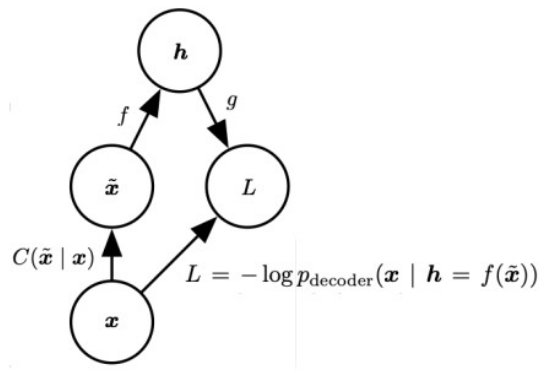
\includegraphics[width=7cm]{Images/denoising-autoencoder.jpg}
    \caption{Denoising autoencoder}
    \label{fig:denoising-autoencoder}
\end{figure}

\noindent Typically we can simply perform gradient-based approximate minimization on the negative log-likelihood: $L = \log(p_{decoder}(x \vert h))$


\subsection{Contractive Autoencoders}

The contractive autoencoder introduces an explicit regularizer on the code $h = f(x)$, encouraging the derivatives of $f$ to be as small as possible:

$$\Omega (h) = \lambda \left| \frac{\partial f (x)}{\partial x} \right|_{F}^{2} $$


The penalty $\Omega (h)$ is the squared Frobenius norm (sum of squared elements) of the Jacobian matrix of partial derivatives associated with the encoder function.

\noindent Contractive autoencoders restrict the model in a way that small changes in the input should result in only small changes in the learned representation. In other words, the autoencoder should be robust to perturbations or noise in the input data. This makes contractive autoencoders able to learn more robust and stable representations compared to traditional autoencoders. Contractive autoencoders also have some practical challenges:

\begin{itemize}
    \item Heavy computational time of the Jacobian for Deep Neural Networks.
    \item The contraction penalty can obtain useless results if we do not impose some sort of scale on the decoder.
\end{itemize}
